\documentclass[a4paper, 12pt]{scrartcl}

% Use Hungarian Locale
\usepackage[magyar]{babel}

% Page layout settings
\usepackage[
  margin=20mm,
  footskip=12mm,
  headheight=20mm,
  % showframe
]{geometry}
\usepackage{fancyhdr}
\usepackage{lastpage}
\usepackage{hyperref}
\pagestyle{fancy}

\renewcommand\footrulewidth{1mm}
\renewcommand\headrulewidth{1mm}

\setlength\parindent{0em}
\setlength\parskip{.67em}

\fancyfoot[C]{\thepage\ / \pageref{LastPage}}
\fancyhead[L]{BMEGEMMBXVE, 1. szorgalmi HF}
\fancyhead[R]{%
  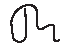
\includegraphics[height = 12px]{static/signature.pdf}
  Sándor Tibor,
  C7XUDE
}

% Math related packages
\usepackage{amsmath}
\usepackage{amssymb}
\usepackage{fontspec}
\usepackage{unicode-math}
\setmainfont{TeX Gyre Termes}
\setsansfont[Scale=MatchUppercase]{TeX Gyre Heros}
\setmathfont{Asana Math}

\usepackage{icomma}
\usepackage{siunitx}
\sisetup{
  per-mode = symbol,
  locale=DE
}

% Vector graphics
\usepackage{tikz}
\usetikzlibrary{
  calc,
  angles,
  quotes,
  backgrounds,
  patterns,
  arrows,
  arrows.meta,
  positioning,
  intersections,
  shapes.geometric,
}

\tikzset{
  dot/.style = {
      circle,
      fill=red!80!gray,
      minimum size=#1,
      draw=black,
      inner sep=0pt, outer sep=0pt
    },
  dot/.default = 5pt,
  gdot/.style = {
      dot,
      fill=white
    },
  dim/.style = {
      latex-latex,
      draw=teal,
      thick
    },
  joint/.style = {
      circle,
      draw=black,
      ultra thick,
      fill=cyan!20,
      minimum size=4mm,
    },
  square/.style = {
      regular polygon,
      regular polygon sides=4
    },
  rod/.style = {
      rectangle,
      draw=black,
      minimum height=6mm,
      minimum width=6mm,
      fill=yellow!10,
      ultra thick,
      midway,
      outer sep=0,
    },
}


% Figure and other imports
\usepackage{pdfpages}
\usepackage{standalone}

% Other dependencies
\usepackage{tabto}
\usepackage{multicol}
\usepackage{xcolor}
\usepackage{float}
\usepackage{array}
\newcolumntype{x}[1]{>{\centering\arraybackslash\hspace{0pt}}p{#1}}
\newcolumntype{X}[1]{>{$}x{#1}<{$}}

\usepackage{luacode}
% noindent
\begin{luacode*}
  utils = require 'lua.utils' 
  variables = require "lua.variables"
\end{luacode*}
% indent

\usepackage{xargs}
\newcommandx{\silv}[3][3=]{\directlua{utils.silv("#1", "#2", "#3")}}
\newcommandx{\sivec}[4][4=]{\directlua{utils.silv1D("#1", "#2", "#3", "#4")}}
\newcommandx{\simat}[5][5=]{\directlua{utils.silv2D("#1", "#2", "#3", "#4", "#5")}}
\newcommandx{\siten}[6][6=]{\directlua{utils.silv3D("#1", "#2", "#3", "#4", "#5", "#6")}}
\newcommand{\lv}[1]{\directlua{utils.lv("#1")}}
\newcommand{\lvmat}[3]{\directlua{utils.lv2D("#1", "#2", "#3")}}
\newcommandx{\lvmth}[6][4=,5=,6=]{\directlua{utils.lv2DTD("#1", "#2", "#3", "#4", "#5", "#6")}}
% \renewcommandx{\num}[2][2=]{\directlua{utils.silv("#1", '', "#2")}}
 % 1112

% Math custom commands
\newcommand\iu{\mathbf{j}}
\newcommand{\rvec}[1]{\mathbfit{#1}}
\newcommand{\uvec}[1]{\widehat{\mathbfit{#1}}}
\newcommand{\rmat}[1]{\mathbf{#1}}

\DeclareMathOperator\atann{atan2}

% Document begins here
\begin{document}

\AddToShipoutPictureFG*{
  \setmainfont{Latin Modern Roman}
  \setmathfont{Latin Modern Math}
  \put(12cm,27.33cm){
    \makebox(7.5cm,1cm){
      \hfill Sándor Tibor
    }
  }
  \put(12cm,26.67cm){
    \makebox(7.5cm,1cm){
      \hfill C7XUDE
    }
  }
  \put(15.45cm,26cm){
    \makebox(7.5cm,1cm){
      \hfill 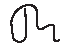
\includegraphics[height=5mm]{./static/signature.pdf} \hfill
    }
  }

  \put(8.8cm,25cm){
    \makebox(15mm,0){\lv{code_1}}
    \makebox(14mm,0){\lv{code_2}}
    \makebox(14mm,0){\lv{code_3}}
    \makebox(14mm,0){\lv{code_4}}
  }

  \put(2.47cm,4.25cm){
    \makebox(41.5mm,0){\lvmth{Ucalc}{1}{1}[2][1000][]}
    \makebox(41.5mm,0){\lvmth{Ucalc}{2}{1}[2][1000][]}
    \makebox(41.5mm,0){\lvmth{Fcalc}{1}{1}[0][.001][]}
    \makebox(41.5mm,0){\lvmth{Fcalc}{2}{1}[0][.001][]}
  }
  \put(2.47cm,3.65cm){
    \makebox(41.5mm,0){\lvmth{Ucalc}{3}{1}[2][1000][]}
    \makebox(41.5mm,0){\lvmth{Ucalc}{4}{1}[2][1000][]}
    \makebox(41.5mm,0){\lvmth{Fcalc}{3}{1}[0][.001][]}
    \makebox(41.5mm,0){\lvmth{Fcalc}{4}{1}[0][.001][]}
  }
  \put(2.47cm,3.05cm){
    \makebox(41.5mm,0){\lvmth{Ucalc}{5}{1}[2][1000][]}
    \makebox(41.5mm,0){\lvmth{Ucalc}{6}{1}[2][1000][]}
    \makebox(41.5mm,0){\lvmth{Fcalc}{5}{1}[0][.001][]}
    \makebox(41.5mm,0){\lvmth{Fcalc}{6}{1}[0][.001][]}
  }
  \put(2.47cm,2.45cm){
    \makebox(41.5mm,0){\lvmth{Ucalc}{7}{1}[2][1000][]}
    \makebox(41.5mm,0){\lvmth{Ucalc}{8}{1}[2][1000][]}
    \makebox(41.5mm,0){\lvmth{Fcalc}{7}{1}[0][.001][]}
    \makebox(41.5mm,0){\lvmth{Fcalc}{8}{1}[0][.001][]}
  }
  \put(2.47cm,1.85cm){
    \makebox(41.5mm,0){\lvmth{Ucalc}{9}{1}[2][1000][]}
    \makebox(41.5mm,0){\lvmth{Ucalc}{10}{1}[2][1000][]}
    \makebox(41.5mm,0){\lvmth{Fcalc}{9}{1}[0][.001][]}
    \makebox(41.5mm,0){\lvmth{Fcalc}{10}{1}[0][.001][]}
  }
}
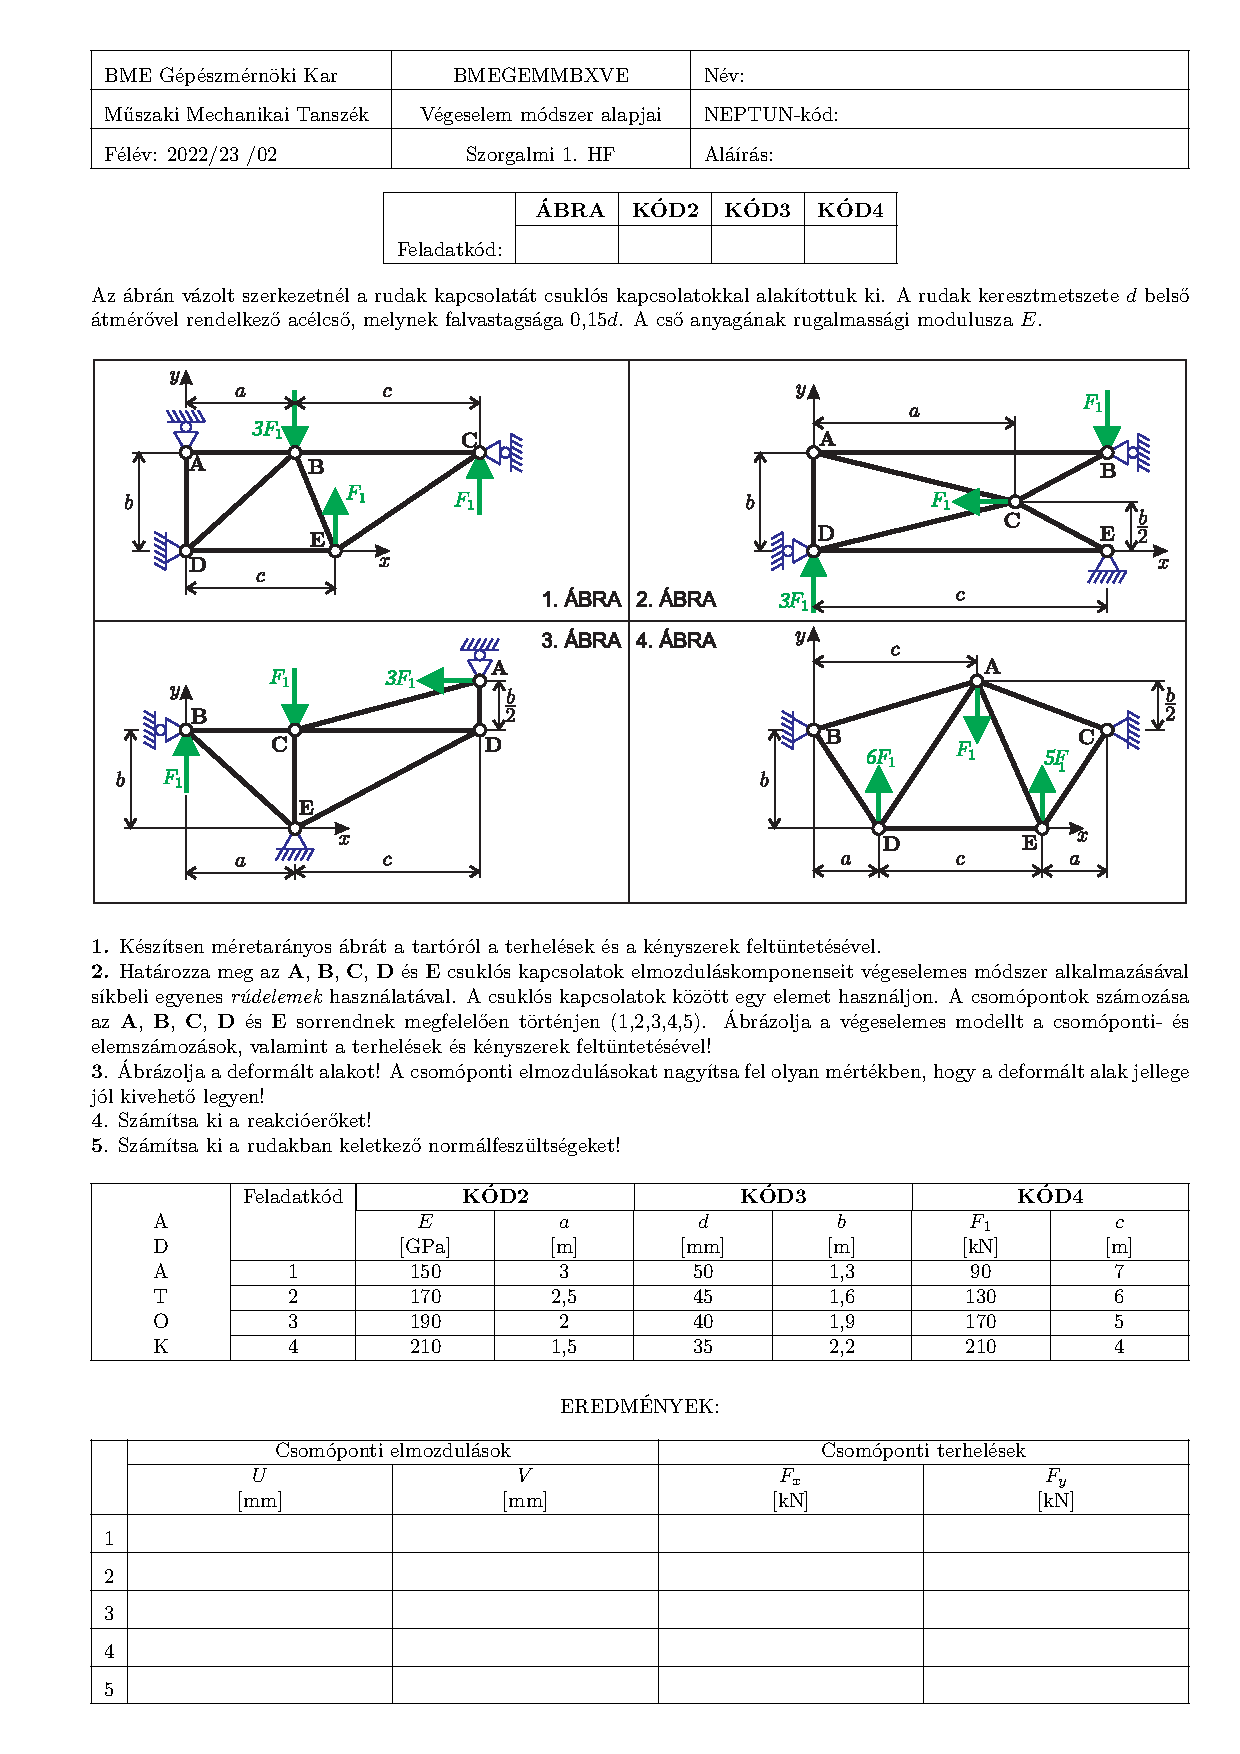
\includepdf[
  pages=-,
  scale=.95,
  pagecommand=\thispagestyle{fancy}
]{./static/titlepage.pdf}
\setmainfont{TeX Gyre Termes}
\setmathfont{Asana Math}


\section{Méretarányos ábra} % (fold)
\label{sec:Méretarányos ábra}

A feladatkódom (\texttt{\lv{code_1}\lv{code_2}\lv{code_3}\lv{code_4}})
alapján a szerkezetet jellemző adatok:
\begin{multicols}{3}
  \begin{itemize}
    \item $a = \silv{a}{m}$,
    \item $d = \silv{d}{mm}$,

    \item $b = \silv{b}{m}$,
    \item $E = \silv{E}{MPa}$,

    \item $c = \silv{c}{m}$,
    \item $F_1 = \silv{F_1}{N}$.
  \end{itemize}
\end{multicols}

A megadott adatok alapján a szerkezetről készített méretarányos vázlat az
\ref{fig:construction}. ábrán látható. A lapon mért $\SI{1}{mm}$ távolság
a valóságban $\SI{1}{m}$-nek felel meg.

\begin{figure}[H]
  \centering
  \includestandalone{construction}
  \caption{Méretarányos ábra a tartóról}
  \label{fig:construction}
\end{figure}

% section section name (end)

\section{Csuklók elmozdulás-komponenseinek számítása} % (fold)
\label{sec:Csuklók elmozdulás-komponenseinek számítása}

A feladat megoldásának megkezdése előtt fontos, hogy először számozzuk be
a szerkezet csomópontjait, és az ezeket összekötő rudakat. Az egyes elemekhez
hozzárendelt sorszámokat a \ref{fig:numbering}. ábra tartalmazza.

\begin{figure}[H]
  \centering
  \includestandalone{numbering}
  \caption{A csomópontok és rudak számozása}
  \label{fig:numbering}
\end{figure}

Határozzuk meg először az elemi merevségi mátrixokat. Egy ilyen mátrix 2D-s
húzott-nyomott rudak esetén az alábbi alakban írhatóak fel:
\def\a{\alpha_i}
\begin{equation}
  \rmat{K}_e^{(i)}
  = \frac{A_i E_i}{L_i}
  \cdot
  \begin{bmatrix}
    \cos^2 \a        & \cos \a \sin \a  & -\cos^2 \a       & -\cos \a \sin \a \\
    \cos \a \sin \a  & \sin^2 \a        & -\cos \a \sin \a & -\sin^2 \a       \\
    -\cos^2 \a       & -\cos \a \sin \a & \cos^2 \a        & \cos \a \sin \a  \\
    -\cos \a \sin \a & -\sin^2 \a       & \cos \a \sin \a  & \sin^2 \a        \\
  \end{bmatrix}.
  \label{eq:Ke}
\end{equation}
\let\a\relax
\def\a{\alpha}

A rudak rugalmassági modulusai ($E_i = E$) már ismertek, viszont $L_i$ hosszuk,
$A_i$ keresztmetszetük, valamint $\alpha_i$ hajlásszögük még nem.

Az összes rúd keresztmetszete azonos, az alábbi képlettel számítható:
\begin{equation}
  A_i = A = \frac{((1,3d)^2 - d^2)\pi}{4} = \silv{A}{mm^2}[2].
  \label{eq:A}
\end{equation}

A rudak hosszai már nem minden esetben azonosak:

\begin{minipage}[c]{.26\linewidth}
  \begin{itemize}
    \item $L_1 = a = \silv{a}{m}$,
    \item $L_2 = b = \silv{b}{m}$,
  \end{itemize}
\end{minipage}%
\begin{minipage}[c]{.33\linewidth}
  \begin{itemize}
    \item $L_3 = L_7 = c = \silv{c}{m}$,
    \item $L_4 = \sqrt{a^2 + b^2} = \simat{L}{m}{4}{1}[2]$,
  \end{itemize}
\end{minipage}%
\begin{minipage}[c]{.38\linewidth}
  \begin{itemize}
    \item $L_5 = \sqrt{(c - a)^2 + b^2} = \simat{L}{m}{5}{1}[2]$,
    \item $L_6 = \sqrt{a^2 + b^2} = \simat{L}{m}{6}{1}[2]$.
  \end{itemize}
\end{minipage}

A vízszintes rudak hajlásszöge $\alpha_1 = \alpha_3 = \alpha_7 = \SI{0}{rad}$,
a többi elemé pedig az $\atann(y; x)$ függvénnyel számítható:
\begin{multicols}{2}
  \begin{itemize}
    \item $\a_2 = -\pi/2 = \simat{alpha}{rad}{2}{1}[4]$,
    \item $\a_4 = \atann \left( -b; -a \right) = \simat{alpha}{rad}{4}{1}[4]$,
    \item $\a_5 = \atann \left( -b; c-a \right) = \simat{alpha}{rad}{5}{1}[4]$,
    \item $\a_6 = \atann \left( -b; -a \right) = \simat{alpha}{rad}{6}{1}[4]$.
  \end{itemize}
\end{multicols}

Az egyes elemek merevségi mátrixai ezen információk alapján már számíthatóak:
\sisetup{
  exponent-mode = scientific,
  round-mode = figures,
  round-precision = 4
}
\begin{equation}
  \sisetup{
    exponent-mode = fixed,
    round-precision = 4
  }
  \begin{split}
    \directlua{utils.fullKei()}
  \end{split}
\end{equation}

Öt csomópontunk van, melyek egyenként két-két szabadsági fokkal rendelkeznek.
($x$ és $y$ irányú elmozdulás) Ez összesen 10 szabadsági fokot jelent.
Rendeljük hozzá a rudakhoz az egyes szabadsági fokokat, melyeket az alábbi
mátrix tartalmazza:

\begin{equation}
  \directlua{utils.printDOFMatrix()}
  \label{eq:DOF}
\end{equation}

A globális merevségi mátrix összeállításakor figyelnünk kell arra, hogy az adott
elem merevségi mátrixának megfelelő elemeit a hozzá tartozó szabadsági fokhoz
tartozó helyhez rendeljük hozzá. Ezt a \ref{fig:table} ábra szemlélteti.
\begin{figure}[H]
  \centering
  \includestandalone{table}
  \caption{A globális merevségi mátrix szemléletes felépítése}
  \label{fig:table}
\end{figure}

A globális merevségi mátrix tehát az alábbi alakot veszi fel:
\sisetup{
  round-precision = 2
}
\begin{equation}
  \sisetup{
    exponent-mode = fixed,
    round-precision = 5
  }
  \scriptsize{
    \rmat K = \begin{bmatrix}
      \directlua{utils.printK(1e-6)}
    \end{bmatrix} \cdot 10^6 \, \mathrm{N/m}
  }.
  \normalsize
  \label{eq:K}
\end{equation}

A merevségi egyenlet felírásához írjuk fel paraméteresen a globális csomóponti
elmozdulásvektort, illetve a globális csomóponti terhelésvektort:
\begin{equation}
  \begin{array}{r c}
    \rvec{U} = & \left[ \begin{array}{*{10}{X{6mm}}}
                            U_1 & V_1 & U_2 & V_2 & U_3 & V_3 & U_4 & V_4 & U_5 & V_5
                          \end{array}
      \right]^\mathsf{T}\text{,}
    \\[2mm]
    \rvec{F} = & \left[ \begin{array}{*{10}{X{6mm}}}
                            F_{1x} & F_{1y} & F_{2x} & F_{2y} & F_{3x} & F_{3y} & F_{4x} & F_{4y} & F_{5x} & F_{5y}
                          \end{array}
      \right]^\mathsf{T}.
  \end{array}
  \label{eq:UF}
\end{equation}

A kényszerek ismeretében tudjuk, hogy az (1)-es csomópont elmozdulása $y$,
(3)-as csomópont elmozdulása $x$, a (4)-es csomópont elmozdulása pedig $x$
és $y$ irányban is gátolt, vagyis: $V_1 = U_3 = U_4 = V_4 = 0$.
Behelyettesítve:
\begin{equation}
  \rvec U = \left[\begin{array}{*{10}{X{6mm}}}
      U_1 & 0 & U_2 & V_2 & 0 & V_3 & 0 & 0 & U_5 & V_5
    \end{array}\right]^\mathsf{T}
  .
  \label{eq:U}
\end{equation}

A terhelésvektor néhány komponense is ismert. A külső terhelések alapján:
$F_{2y} = -3 F_1$, $F_{3y} = F_1$, $F_{5y} = F_1$. Tudjuk továbbá hogy
$F_{1x} = F_{2x} = F_{5x} = 0$, hiszen ezek a csomópontok ilyen irányban
terheletlenek:
\begin{equation}
  \rvec F = \left[\begin{array}{*{10}{X{7.75mm}}}
      0 & F_{1y} & 0 & \text{-}3F_1 & F_{3x} & F_1 & F_{4x} & F_{4y} & 0 & F_1
    \end{array}\right]^\mathsf{T}
  .
  \label{eq:F}
\end{equation}

Ezen adatok ismeretében már fel tudjuk írni a kondenzált merevségi egyenletet,
melyet úgy kapunk meg, hogy az elmozdulásban gátolt irányokhoz tartozó sorokat
és oszlopokat töröljük az eredeti, globális merevségi egyenletből:
\begin{equation}
  \underbrace{\begin{bmatrix}
      \directlua{utils.printKkond()}
    \end{bmatrix}}_{\widehat{\rmat K}}
  \underbrace{\begin{bmatrix}
      U_1 \\ U_2 \\ V_2 \\ V_3 \\ U_5 \\ V_5
    \end{bmatrix}}_{\widehat{\rvec U}}
  =
  \sisetup{
    exponent-mode = fixed,
    round-precision = 3
  }
  \underbrace{\begin{bmatrix}
      \directlua{utils.printFkond()}
    \end{bmatrix}}_{\widehat{\rvec F}}
  .
  \label{eq:cond}
\end{equation}

Mivel $\widehat{\rmat K}$ mátrix reguláris, ezért az egyenletrendszer
mátrix-invertálással megoldható, vagyis:
\begin{equation}
  \widehat{\rvec U} =
  \underbrace{\begin{bmatrix}
      \directlua{utils.printInverted()}
    \end{bmatrix}}_{\widehat{\rmat K}^{-1}}
  \sisetup{
    exponent-mode = fixed,
    round-precision = 3
  }
  \underbrace{\begin{bmatrix}
      \directlua{utils.printFkond()}
    \end{bmatrix}}_{\widehat{\rvec F}}
  .
  \label{eq:inverted}
\end{equation}

Az egyenlet megoldása numerikusan:
\sisetup{round-precision = 3}
\begin{equation}
  \widehat{\rvec U} = \begin{bmatrix}
    \directlua{utils.printUkond(1)}
  \end{bmatrix} \, \mathrm{m}
  =
  \sisetup{exponent-mode = fixed}
  \begin{bmatrix}
    \directlua{utils.printUkond(1000)}
  \end{bmatrix} \, \mathrm{mm}.
  \label{eq:numericCond}
\end{equation}

A globális elmozdulásvektorba visszahelyettesítve:
\begin{equation}
  {\rvec U} = \begin{bmatrix}
    \directlua{utils.printUcalc(1)}
  \end{bmatrix} \, \mathrm{m}
  =
  \sisetup{
    exponent-mode = fixed,
    round-precision = 3
  }
  \begin{bmatrix}
    \directlua{utils.printUcalc(1000)}
  \end{bmatrix} \, \mathrm{mm}.
  \label{eq:Ucalc}
\end{equation}

% section section name (end)



\section{A deformált alak ábrázolása} % (fold)
\label{sec:A deformált alak ábrázolása}

Az $\rmat U$ vektor ismeretében már ábrázolhatjuk a csomópontok új koordinátáit.
A \ref{fig:deformed} ábra az elmozdulások ötszörös nagyításával szemlélteti a
szerkezet deformált alakját.

\begin{figure}[H]
  \centering
  \includestandalone{deformed}
  \caption{A deformált alak szemléltetése}
  \label{fig:deformed}
\end{figure}

% section section name (end)



\section{A reakcióerők meghatározása} % (fold)
\label{sec:A reakcióerők meghatározása}

Ha a merevségi egyenletbe visszahelyettesítjük a már ismert elmozdulási vektort,
akkor megkaphatjuk a terhelési vektort numerikusan:
\begin{equation}
  \rvec F = \rmat K \rvec U =
  \sisetup{
    exponent-mode = fixed,
    round-precision = 3
  }
  \begin{bmatrix}
    \directlua{utils.printFcalc(1)}
  \end{bmatrix}
  =
  \underbrace{\begin{bmatrix}
      \directlua{utils.printF(1)}
    \end{bmatrix}}_\text{terhelés}
  +
  \underbrace{\begin{bmatrix}
      \directlua{utils.printFreacc(1)}
    \end{bmatrix}}_\text{reakció}
  \, \mathrm{N}.
  \label{eq:Fcalc}
\end{equation}

A reakcióerők tehát a következőek:
\begin{equation}
  \sisetup{
    exponent-mode = fixed,
    round-precision = 3
  }
  \begin{split}
    F_{3x} &= \simat{Fcalc}{N}{5}{1}\text,
    \\
    F_{4x} &= \simat{Fcalc}{N}{7}{1}\text,
    \\
    F_{4y} &= \simat{Fcalc}{N}{8}{1}.
  \end{split}
\end{equation}

% section sec:A reakcióerők meghatározása (end)



\section{Normálfeszültségek számítása} % (fold)
\label{sec:Normálfeszültségek számítása}

Határozzuk meg először az elemekhez tartozó lokális elmozdulásvektorokat,
melyek elemei a globális elmozdulásvektor megfelelő elemeivel egyeznek meg:
\begin{equation}
  \begin{aligned}
    \directlua{utils.fullUei()}
  \end{aligned}
\end{equation}

Az alakváltozások számításához definiáljuk a $\rvec B$ sorvektort az alábbi módon:
\begin{equation}
  \rvec B_i := \frac{1}{L_i} \left[\begin{array}{*{4}{X{14mm}}}
      -\cos \a_i &
      -\sin \a_i &
      \cos \a_i  &
      \sin \a_i
    \end{array}\right].
  \label{eq:B}
\end{equation}

Az $\varepsilon_i$ alakváltozások és az $\rvec U_i$ vektorok közötti kapcsolat
az alábbi egyenlettel írható fel:
\begin{equation}
  \varepsilon_i = \rvec B_i \cdot \rvec U_i.
  \label{eq:eps}
\end{equation}

\sisetup{
  exponent-mode = fixed,
  round-precision = 4
}
Ezen értékek numerikusan:
\begin{multicols}{3}
  \begin{itemize}
    \item $\varepsilon_1 = \varepsilon_2 = 0,$
    \item $\varepsilon_3 = \sivec{epsilon}{}{3}[6]$,
    \item $\varepsilon_4 = \sivec{epsilon}{}{4}[6]$,
    \item $\varepsilon_5 = \sivec{epsilon}{}{5}[6]$,
    \item $\varepsilon_6 = \sivec{epsilon}{}{6}[6]$,
    \item $\varepsilon_7 = \sivec{epsilon}{}{7}[6]$.
  \end{itemize}
\end{multicols}

A normálfeszültségek és a mérnöki alakváltozások között a Hooke-törvény teremt
kapcsolatot:
\begin{equation}
  \sigma_i = E_i \cdot \varepsilon_i.
  \label{eq:Hooke}
\end{equation}

\sisetup{round-precision = 4}
A feszültségek numerikusan:
\begin{multicols}{3}
  \begin{itemize}
    \item $\sigma_1 = \sigma_2 = \SI{0}{MPa},$
    \item $\sigma_3 = \sivec{sigma}{MPa}{3}$,
    \item $\sigma_4 = \sivec{sigma}{MPa}{4}$,
    \item $\sigma_5 = \sivec{sigma}{MPa}{5}$,
    \item $\sigma_6 = \sivec{sigma}{MPa}{6}$,
    \item $\sigma_7 = \sivec{sigma}{MPa}{7}$.
  \end{itemize}
\end{multicols}

% section section name (end)

% \clearpage

% \tableofcontents

\vfill

\section*{Felhasznált szoftverek}

\begin{itemize}
  \item \href{https://neovim.io}{\texttt{Neovim}}
        \tabto{3.9cm} – \tabto{4.7cm}
        Open Source szövegszerkesztő

  \item \texttt{Lua\LaTeX}
        \tabto{3.9cm} – \tabto{4.7cm}
        \LaTeX{} fordító

  \item \texttt{Ti\textit{k}Z}
        \tabto{3.9cm} – \tabto{4.7cm}
        Vektorgrafika

  \item \texttt{lua}
        \tabto{3.9cm} – \tabto{4.7cm}
        Számítások elvégzése
\end{itemize}

A házi feladat teljes forráskódja -- beleértve a számolást és dokumentációt --
megtekinthető az alábbi linken:
\texttt{\href{https://github.com/tibi1220/VEM-1SZHF}{https://github.com/tibi1220/VEM-1SZHF}}

\end{document}
